% Options for packages loaded elsewhere
\PassOptionsToPackage{unicode}{hyperref}
\PassOptionsToPackage{hyphens}{url}
%
\documentclass[
  letterpaper,
  ignorenonframetext,
  aspectratio=43,
  handout,
  12pt]{beamer}
\usepackage{pgfpages}
\setbeamertemplate{caption}[numbered]
\setbeamertemplate{caption label separator}{: }
\setbeamercolor{caption name}{fg=normal text.fg}
\beamertemplatenavigationsymbolsempty
% Prevent slide breaks in the middle of a paragraph
\widowpenalties 1 10000
\raggedbottom
\setbeamertemplate{part page}{
  \centering
  \begin{beamercolorbox}[sep=16pt,center]{part title}
    \usebeamerfont{part title}\insertpart\par
  \end{beamercolorbox}
}
\setbeamertemplate{section page}{
  \centering
  \begin{beamercolorbox}[sep=12pt,center]{part title}
    \usebeamerfont{section title}\insertsection\par
  \end{beamercolorbox}
}
\setbeamertemplate{subsection page}{
  \centering
  \begin{beamercolorbox}[sep=8pt,center]{part title}
    \usebeamerfont{subsection title}\insertsubsection\par
  \end{beamercolorbox}
}
\AtBeginPart{
  \frame{\partpage}
}
\AtBeginSection{
  \ifbibliography
  \else
    \frame{\sectionpage}
  \fi
}
\AtBeginSubsection{
  \frame{\subsectionpage}
}
\usepackage{amsmath,amssymb}
\usepackage{lmodern}
\usepackage{ifxetex,ifluatex}
\ifnum 0\ifxetex 1\fi\ifluatex 1\fi=0 % if pdftex
  \usepackage[T1]{fontenc}
  \usepackage[utf8]{inputenc}
  \usepackage{textcomp} % provide euro and other symbols
\else % if luatex or xetex
  \usepackage{unicode-math}
  \defaultfontfeatures{Scale=MatchLowercase}
  \defaultfontfeatures[\rmfamily]{Ligatures=TeX,Scale=1}
\fi
\usetheme[]{metropolis}
% Use upquote if available, for straight quotes in verbatim environments
\IfFileExists{upquote.sty}{\usepackage{upquote}}{}
\IfFileExists{microtype.sty}{% use microtype if available
  \usepackage[]{microtype}
  \UseMicrotypeSet[protrusion]{basicmath} % disable protrusion for tt fonts
}{}
\makeatletter
\@ifundefined{KOMAClassName}{% if non-KOMA class
  \IfFileExists{parskip.sty}{%
    \usepackage{parskip}
  }{% else
    \setlength{\parindent}{0pt}
    \setlength{\parskip}{6pt plus 2pt minus 1pt}}
}{% if KOMA class
  \KOMAoptions{parskip=half}}
\makeatother
\usepackage{xcolor}
\IfFileExists{xurl.sty}{\usepackage{xurl}}{} % add URL line breaks if available
\IfFileExists{bookmark.sty}{\usepackage{bookmark}}{\usepackage{hyperref}}
\hypersetup{
  hidelinks,
  pdfcreator={LaTeX via pandoc}}
\urlstyle{same} % disable monospaced font for URLs
\newif\ifbibliography
\usepackage{graphicx}
\makeatletter
\def\maxwidth{\ifdim\Gin@nat@width>\linewidth\linewidth\else\Gin@nat@width\fi}
\def\maxheight{\ifdim\Gin@nat@height>\textheight\textheight\else\Gin@nat@height\fi}
\makeatother
% Scale images if necessary, so that they will not overflow the page
% margins by default, and it is still possible to overwrite the defaults
% using explicit options in \includegraphics[width, height, ...]{}
\setkeys{Gin}{width=\maxwidth,height=\maxheight,keepaspectratio}
% Set default figure placement to htbp
\makeatletter
\def\fps@figure{htbp}
\makeatother
\setlength{\emergencystretch}{3em} % prevent overfull lines
\providecommand{\tightlist}{%
  \setlength{\itemsep}{0pt}\setlength{\parskip}{0pt}}
\setcounter{secnumdepth}{-\maxdimen} % remove section numbering
\usepackage{pgfpages}
\pgfpagesuselayout{2 on 1}
\providecommand{\tightlist}{%
\setlength{\itemsep}{0pt}\setlength{\parskip}{0pt}}
\makeatletter
\makeatother
\let\Oldincludegraphics\includegraphics
\renewcommand{\includegraphics}[2][]{\Oldincludegraphics[width=\textwidth,height=0.7\textheight,keepaspectratio]{#2}}
\ifluatex
  \usepackage{selnolig}  % disable illegal ligatures
\fi

\author{}
\date{}

\begin{document}

\begin{frame}
Lecture 3 - Coordinate Transformation

Dr.~Nicholas Smith

Wichita State University, Department of Aerospace Engineering

February 9, 2021
\end{frame}

\begin{frame}{schedule}
\protect\hypertarget{schedule}{}
\begin{itemize}
\tightlist
\item
  Feb 9 - Coordinate Transformation
\item
  Feb 11 - 1D Micromechanics (HW1 Due)
\item
  Feb 16 - Mean-field
\item
  Feb 18 - Orientation Averaging (HW2 Due)
\end{itemize}
\end{frame}

\begin{frame}{outline}
\protect\hypertarget{outline}{}
\begin{itemize}
\tightlist
\item
  transformation
\item
  engineering notation
\end{itemize}
\end{frame}

\hypertarget{transformation}{%
\section{transformation}\label{transformation}}

\begin{frame}{general coordinate transformation}
\protect\hypertarget{general-coordinate-transformation}{}
\begin{itemize}
\tightlist
\item
  Coordinate transformation can become much more complicated in three
  dimensions, and with higher-order tensors
\item
  It is convenient to define a general form of the coordinate
  transformation in index notation
\item
  We define \(Q_{ij}\) as the cosine of the angle between the
  \(x_i^\prime\) axis and the \(x_j\) axis.
\item
  This is also referred to as the ``direction cosine''
\end{itemize}

\[Q_{ij} = \cos(x_i^\prime, x_j)\]
\end{frame}

\begin{frame}{mental and emotional health warning}
\protect\hypertarget{mental-and-emotional-health-warning}{}
\begin{itemize}
\tightlist
\item
  Different textbooks flip the definition of \(Q_{ij}\) (Elasticity and
  Continuum texts have opposite definitions, for example)
\item
  The result gives the transpose
\item
  Always use equations (next slide) from the same source as your
  \(Q_{ij}\) definition
\end{itemize}
\end{frame}

\begin{frame}{general coordinate transformation}
\protect\hypertarget{general-coordinate-transformation-1}{}
\begin{itemize}
\tightlist
\item
  We can transform any-order tensor using \(Q_{ij}\)
\item
  Vectors (first-order tensors): \(v_i^\prime = Q_{ij} v_j\)
\item
  Matrices (second-order tensors):
  \(\sigma_{ij}^\prime = Q_{im}Q_{jn} \sigma_{mn}\)
\item
  Fourth-order tensors:
  \(C_{ijkl}^\prime = Q_{im}Q_{jn}Q_{ko}Q_{lp} C_{mnop}\)
\end{itemize}
\end{frame}

\begin{frame}{transformation}
\protect\hypertarget{transformation-1}{}
\begin{itemize}
\tightlist
\item
  We can use this form on our 2D transformation example
\end{itemize}

\[\begin{aligned}
  Q_{ij} &= \cos (x_i^\prime, x_j)\\
&=
  \begin{bmatrix}
  \cos (x_1^\prime, x_1) & \cos (x_1^\prime, x_2)\\
  \cos (x_2^\prime, x_1) & \cos (x_2^\prime, x_2)
  \end{bmatrix}\\
  &= \begin{bmatrix}
  \cos \theta & \cos (90-\theta)\\
  \cos (90+\theta) & \cos \theta
  \end{bmatrix} \\
  &= \begin{bmatrix}
  \cos \theta & \sin \theta \\
  -\sin \theta & \cos \theta
  \end{bmatrix}
\end{aligned}\]
\end{frame}

\begin{frame}{general coordinate transformation}
\protect\hypertarget{general-coordinate-transformation-2}{}
\begin{itemize}
\tightlist
\item
  We can similarly use \(Q_{ij}\) to find tensors in the original
  coordinate system
\item
  Vectors (first-order tensors): \(v_j = Q_{ij} v_i^\prime\)
\item
  Matrices (second-order tensors):
  \(\sigma_{mn} = Q_{im}Q_{jn} \sigma_{ij}^\prime\)
\item
  Fourth-order tensors:
  \(C_{mnop} = Q_{im}Q_{jn}Q_{ko}Q_{lp} C_{ijkl}^\prime\)
\end{itemize}
\end{frame}

\begin{frame}{general coordinate transformation}
\protect\hypertarget{general-coordinate-transformation-3}{}
\begin{itemize}
\tightlist
\item
  We can derive some interesting properties of the transformation
  tensor, \(Q_{ij}\)
\item
  We know that \(v_i^\prime = Q_{ij} v_j\) and that
  \(v_j = Q_{ij} v_i^\prime\)
\item
  If we substitute (changing the appropriate indexes) we find:
\item
  \(v_j = Q_{ij} Q_{ik} v_k\)
\item
  We can now use the Kronecker Delta to substitute
  \(v_j = \delta_{jk}v_k\)
\item
  \(\delta_{jk}v_k = Q_{ij} Q_{ik} v_k\)
\end{itemize}
\end{frame}

\hypertarget{engineering-notation}{%
\section{engineering notation}\label{engineering-notation}}

\begin{frame}{engineering notation}
\protect\hypertarget{engineering-notation-1}{}
\[\begin{bmatrix}
  \sigma_{11} \\
\sigma_{22} \\
\sigma_{33} \\
\sigma_{23} \\
\sigma_{13} \\
\sigma_{12}
  \end{bmatrix}
  = \begin{bmatrix}
  C_{1111} & C_{1122} & C_{1133} & C_{1123} & C_{1113} & C_{1112} \\
  C_{1122} & C_{2222} & C_{2233} & C_{2223} & C_{1322} & C_{1222} \\
  C_{1133} & C_{2233} & C_{3333} & C_{2333} & C_{1333} & C_{1233} \\
  C_{1123} & C_{2223} & C_{2333} & C_{2323} & C_{1323} & C_{1223} \\
  C_{1113} & C_{1322} & C_{1333} & C_{1323} & C_{1313} & C_{1213} \\
  C_{1112} & C_{1222} & C_{1233} & C_{1223} & C_{1213} & C_{1212}
  \end{bmatrix}\begin{bmatrix}
  E_{11} \\
E_{22} \\
E_{33} \\
2E_{23} \\
2E_{13} \\
2E_{12}
\end{bmatrix}\]
\end{frame}

\begin{frame}{orthotropic symmetry}
\protect\hypertarget{orthotropic-symmetry}{}
\[\small \begin{bmatrix}
  \sigma_{11}\\
\sigma_{22} \\
\sigma_{33} \\
\sigma_{23} \\
\sigma_{13} \\
\sigma_{12}
  \end{bmatrix}
  = \begin{bmatrix}
  C_{1111} & C_{1122} & C_{1133} & 0 & 0 & 0 \\
  C_{1122} & C_{2222} & C_{2233} & 0 & 0 & 0 \\
  C_{1133} & C_{2233} & C_{3333} & 0 & 0 & 0 \\
  0 & 0 & 0 & C_{2323} & 0 & 0 \\
  0 & 0 & 0 & 0 & C_{1313} & 0 \\
  0 & 0 & 0 & 0 & 0 & C_{1212}
  \end{bmatrix}\begin{bmatrix}
  E_{11}\\
E_{22} \\
E_{33} \\
2E_{23} \\
2E_{13} \\
2E_{12}
\end{bmatrix}\]
\end{frame}

\begin{frame}{transversely isotropic symmetry}
\protect\hypertarget{transversely-isotropic-symmetry}{}
\[\small \begin{bmatrix}
  \sigma_{11}\\
\sigma_{22} \\
\sigma_{33} \\
\sigma_{23} \\
\sigma_{13} \\
\sigma_{12}
  \end{bmatrix}
  = \begin{bmatrix}
  C_{1111} & C_{1122} & C_{1133} & 0 & 0 & 0 \\
  C_{1122} & C_{1111} & C_{1133} & 0 & 0 & 0 \\
  C_{1133} & C_{1133} & C_{3333} & 0 & 0 & 0 \\
  0 & 0 & 0 & C_{1313} & 0 & 0 \\
  0 & 0 & 0 & 0 & C_{1313} & 0 \\
  0 & 0 & 0 & 0 & 0 & 1/2(C_{1111}-C_{2222})
  \end{bmatrix}\begin{bmatrix}
  E_{11}\\
E_{22} \\
E_{33} \\
2E_{23} \\
2E_{13} \\
2E_{12}
\end{bmatrix}\]
\end{frame}

\begin{frame}{isotropic symmetry}
\protect\hypertarget{isotropic-symmetry}{}
\[\scriptsize \begin{bmatrix}
  \sigma_{11}\\
\sigma_{22} \\
\sigma_{33} \\
\sigma_{23} \\
\sigma_{13} \\
\sigma_{12}
  \end{bmatrix}
  = \frac{E}{(1+\nu)(1-2\nu)}\begin{bmatrix}
  1-\nu & \nu & \nu & 0 & 0 & 0 \\
  \nu & 1-\nu & \nu & 0 & 0 & 0 \\
  \nu & \nu & 1-\nu & 0 & 0 & 0 \\
  0 & 0 & 0 & \frac{1}{2}(1-2\nu) & 0 & 0 \\
  0 & 0 & 0 & 0 & \frac{1}{2}(1-2\nu) & 0 \\
  0 & 0 & 0 & 0 & 0 & \frac{1}{2}(1-2\nu)
  \end{bmatrix}\begin{bmatrix}
  E_{11}\\
E_{22} \\
E_{33} \\
2E_{23} \\
2E_{13} \\
2E_{12}
\end{bmatrix}\]
\end{frame}

\begin{frame}{transformation}
\protect\hypertarget{transformation-2}{}
\begin{itemize}
\item
  We know that
\item
  \[\sigma_{mn} = Q_{im}Q_{jn} \sigma_{ij}^\prime\]
\item
  We can expand this to write in terms of engineering stress
\item
  We will expand only two terms, as they show the general pattern for
  all 6
\end{itemize}
\end{frame}

\begin{frame}{stress transformation}
\protect\hypertarget{stress-transformation}{}
\[\small{\begin{aligned}
    \sigma_{1}^\prime &= \sigma_{11}^\prime =  Q_{11}Q_{11} \sigma_{11} + Q_{11}Q_{12} \sigma_{12} + Q_{11}Q_{13}\sigma_{13}\\
    & + Q_{12}Q_{11} \sigma_{21} + Q_{12}Q_{12} \sigma_{22} + Q_{12}Q_{13}\sigma_{23}\\
    & + Q_{13}Q_{11} \sigma_{31} + Q_{13}Q_{12} \sigma_{32} + Q_{13}Q_{13}\sigma_{33}
\end{aligned}}\]

\[\small{\begin{aligned}
    \sigma_{1}^\prime &= Q_{11}^2 \sigma_{1} + Q_{12}^2 \sigma_{2} + Q_{13}^2\sigma_{3}\\
    & + 2 Q_{11}Q_{12} \sigma_{6} + 2Q_{11}Q_{13}\sigma_{5} + 2Q_{12}Q_{13}\sigma_{4}
\end{aligned}}\]
\end{frame}

\begin{frame}{stress transformation}
\protect\hypertarget{stress-transformation-1}{}
\[\begin{aligned}
 \sigma_{4}^\prime &= \sigma_{23}^\prime =  Q_{21}Q_{31} \sigma_{11} + Q_{21}Q_{32} \sigma_{12} + Q_{21}Q_{33}\sigma_{13}\\
 &+ Q_{22}Q_{31} \sigma_{21} + Q_{22}Q_{32} \sigma_{22} + Q_{22}Q_{33}\sigma_{23}\\
 &+ Q_{23}Q_{31} \sigma_{31} + Q_{23}Q_{32} \sigma_{32} + Q_{23}Q_{33}\sigma_{33}
\end{aligned}\]

\[\begin{aligned}
 \sigma_{4}^\prime &= Q_{21}Q_{31} \sigma_{1} + Q_{22}Q_{32} \sigma_{22} + Q_{23}Q_{33}\sigma_{3}\\
 &+ (Q_{21}Q_{32}+Q_{22}Q_{31}) \sigma_{6} + (Q_{21}Q_{33}+Q_{23}Q_{31})\sigma_{5}\\
 &+ (Q_{22}Q_{33}+Q_{23}Q_{32})\sigma_{4}
\end{aligned}\]
\end{frame}

\begin{frame}{stress transformation}
\protect\hypertarget{stress-transformation-2}{}
\begin{itemize}
\tightlist
\item
  We often write \(\sigma^\prime =R_\sigma \sigma\) for engineering
  notation
\end{itemize}

\[\scriptsize{R_\sigma = \begin{bmatrix}
      Q_{11}^2 & Q_{12}^2 & Q_{13}^2 & 2Q_{12}Q_{13} & 2 Q_{11} Q_{13} & 2Q_{11}Q_{12}\\
      Q_{21}^2 & Q_{22}^2 & Q_{23}^2 & 2Q_{22}Q_{23} & 2 Q_{21} Q_{23} & 2Q_{21}Q_{22}\\
      Q_{31}^2 & Q_{32}^2 & Q_{33}^2 & 2Q_{32}Q_{33} & 2 Q_{31} Q_{33} & 2Q_{31}Q_{32}\\
      Q_{21}Q_{31} & Q_{22}Q_{32} & Q_{23}Q_{33} & Q_{23}Q_{32} + Q_{22}Q_{33} & Q_{23}Q_{31} + Q_{21}Q_{33} & Q_{22}Q_{31} + Q_{21}Q_{32}\\
      Q_{11}Q_{31} & Q_{12}Q_{32} & Q_{13}Q_{33} & Q_{13}Q_{32} + Q_{12}Q_{33} & Q_{13}Q_{31} + Q_{11}Q_{33} & Q_{12}Q_{31} + Q_{11}Q_{32}\\
      Q_{11}Q_{21} & Q_{12}Q_{22} & Q_{13}Q_{23} & Q_{13}Q_{22} + Q_{12}Q_{23} & Q_{13}Q_{21} + Q_{11}Q_{23} & Q_{12}Q_{21} + Q_{11}Q_{22}
\end{bmatrix}}\]
\end{frame}

\begin{frame}{strain transformation}
\protect\hypertarget{strain-transformation}{}
\begin{itemize}
\tightlist
\item
  We can follow the exact same procedure to transform strain
\item
  The values are almost the same, notice the highlighted terms
\end{itemize}

\[ \tiny{R_\epsilon = \begin{bmatrix}
    Q_{11}^2 & Q_{12}^2 & Q_{13}^2 & {    \colorbox{red}{$ Q_{12}Q_{13} $}} &  {    \colorbox{red}{$ Q_{11} Q_{13} $}} & {    \colorbox{red}{$ Q_{11}Q_{12} $}}\\
    Q_{21}^2 & Q_{22}^2 & Q_{23}^2 & {    \colorbox{red}{$ Q_{22}Q_{23} $}} &  {    \colorbox{red}{$ Q_{21} Q_{23} $}} & {    \colorbox{red}{$ Q_{21}Q_{22} $}}\\
    Q_{31}^2 & Q_{32}^2 & Q_{33}^2 & {    \colorbox{red}{$ Q_{32}Q_{33} $}} &  {    \colorbox{red}{$ Q_{31} Q_{33} $}} & {    \colorbox{red}{$ Q_{31}Q_{32} $}}\\
    {    \colorbox{red}{$ Q_{21}Q_{31} $}} & {    \colorbox{red}{$ Q_{22}Q_{32} $}} & {    \colorbox{red}{$ Q_{23}Q_{33} $}} & Q_{23}Q_{32} + Q_{22}Q_{33} & Q_{23}Q_{31} + Q_{21}Q_{33} & Q_{22}Q_{31} + Q_{21}Q_{32}\\
    {    \colorbox{red}{$ Q_{11}Q_{31} $}} & {    \colorbox{red}{$ Q_{12}Q_{32} $}} & {    \colorbox{red}{$ Q_{13}Q_{33} $}} & Q_{13}Q_{32} + Q_{12}Q_{33} & Q_{13}Q_{31} + Q_{11}Q_{33} & Q_{12}Q_{31} + Q_{11}Q_{32}\\
    {    \colorbox{red}{$ Q_{11}Q_{21} $}} & {    \colorbox{red}{$ Q_{12}Q_{22} $}} & {    \colorbox{red}{$ Q_{13}Q_{23} $}} & Q_{13}Q_{22} + Q_{12}Q_{23} & Q_{13}Q_{21} + Q_{11}Q_{23} & Q_{12}Q_{21} + Q_{11}Q_{22}
\end{bmatrix}}\]
\end{frame}

\begin{frame}{stiffness transformation}
\protect\hypertarget{stiffness-transformation}{}
\begin{itemize}
\tightlist
\item
  We can now formulate the transformation of the stiffness matrix. We
  know that
\end{itemize}

\[ \sigma^\prime = R \sigma_\sigma = C^\prime E^\prime\]

\begin{itemize}
\tightlist
\item
  And since \(\sigma=CE\), we can say
\end{itemize}

\[ R_\sigma CE = C^\prime E^\prime\] - Now we know that
\(E^\prime = R_E E\), so we substitute that to find

\[ R_\sigma CE = C^\prime R_E E\]
\end{frame}

\begin{frame}{stiffness transformation}
\protect\hypertarget{stiffness-transformation-1}{}
\begin{itemize}
\tightlist
\item
  We can right multiply both sides by \emph{E}-1 to cancel \emph{E}
\item
  Then we can right multiply both sides by \emph{R}\emph{E}-1 to get
  \emph{C}' by itself
\end{itemize}

\[C^\prime = R_\sigma C (R_E)^{-1}\]

\begin{itemize}
\tightlist
\item
  Note that \(R_E^{-1} = R_\sigma^T\)
\end{itemize}
\end{frame}

\begin{frame}{conventions}
\protect\hypertarget{conventions}{}
\begin{itemize}
\tightlist
\item
  There are two things that can be very confusing when transforming
  engineering stiffness
\item
  First, while I have used the most standard ordering of stress/strain
  terms, not everyone uses the same order
\item
  Second, the equations used here are for engineering strain (which is
  the most common)
\item
  However, tensorial strain may also be used, in which case
  \(R_\sigma = R_E\), but that adds other complications
\end{itemize}
\end{frame}

\hypertarget{one-dimensional-micromechanics}{%
\section{one dimensional
micromechanics}\label{one-dimensional-micromechanics}}

\begin{frame}{one dimensional micromechanics}
\protect\hypertarget{one-dimensional-micromechanics-1}{}
\begin{itemize}
\tightlist
\item
  Some simple one-dimensional micromechanics models are useful as
  bounding cases
\item
  The first micromechancis models were developed by Voigt and Reuss
\item
  These provide a type of bound to possible solutions
\item
  Some improvements were made using the method of cells
\end{itemize}
\end{frame}

\begin{frame}{equivalent solid}
\protect\hypertarget{equivalent-solid}{}
\begin{itemize}
\tightlist
\item
  The goal of all micromechanics models is to use the known properties
  of constituents to find the large-scale behavior
\item
  We can find this by averaging the stress and strain tensors over the
  volume of some RVE
\end{itemize}

\[\begin{aligned}
  \bar{\sigma}_{ij} &= \frac{1}{V}\\int_V \sigma_{ij}(x,y,z) dV\\
  \bar{\epsilon}_{ij} &= \frac{1}{V}\\int_V \epsilon_{ij}(x,y,z) dV
\end{aligned}\]
\end{frame}

\begin{frame}{equivalent solid}
\protect\hypertarget{equivalent-solid-1}{}
\begin{itemize}
\tightlist
\item
  If we have only two phases (fiber and matrix), and we use engineering
  notation, this average can be expressed as
\end{itemize}

\[\begin{aligned}
  \bar{\sigma}_{i} &= \frac{1}{V}\\left(\\int_{V^f} \sigma^f_{i}(x,y,z) dV  + \\int_{V^m} \sigma^m_{i}(x,y,z) dV\\right)\\
  \bar{\epsilon}_{i} &= \frac{1}{V}\\left(\\int_{V^f} \epsilon^f_{i}(x,y,z) dV  + \\int_{V^m} \epsilon^m_{i}(x,y,z) dV\\right)
\end{aligned}\]
\end{frame}

\begin{frame}{equivalent solid}
\protect\hypertarget{equivalent-solid-2}{}
\begin{itemize}
\tightlist
\item
  We also know that in the fiber and matrix, respectively, Hooke's Law
  still holds
\end{itemize}

\[ \sigma_i = C_{ij} \epsilon_j \]

\begin{itemize}
\tightlist
\item
  And this must be true for the average as well
\end{itemize}

\[\bar{\sigma}_i = C_{ij} \bar{\epsilon}_j\]
\end{frame}

\begin{frame}{voigt}
\protect\hypertarget{voigt}{}
\begin{itemize}
\tightlist
\item
  Voigt considered a two-phase composite with a uniform strain imposed
  on both phases
\item
  The uniform strain assumption means that
\end{itemize}

\[ \epsilon_i^f = \epsilon_i^m = \epsilon_i\]

\begin{itemize}
\tightlist
\item
  While a macroscopically homogeneous strain does not necessarily impose
  a locally homogeneous strain field, Voigt assumed that
\end{itemize}

\[\epsilon_i = \bar{\epsilon}_i\]
\end{frame}

\begin{frame}{voigt}
\protect\hypertarget{voigt-1}{}
\begin{itemize}
\tightlist
\item
  This assumption results in
\end{itemize}

\[\begin{aligned}
  \bar{\sigma}_i &= \frac{1}{V}\\left(\\int_{V^f} C_{ij}^f\bar{\epsilon}_j dV  + \\int_{V^m} C_{ij}^m\bar{\epsilon}_j dV\\right)\\
  \bar{\sigma}_i &= \\left( \frac{V_f}{V} C_{ij}^f + \frac{V_m}{V} C_{ij}^m\\right)\bar{\epsilon}_j
\end{aligned}\]

\begin{itemize}
\tightlist
\item
  This gives the well-known rule of mixtures for \emph{C}\emph{ij}
\end{itemize}

\[C_{ij}^c = \frac{V_f}{V} C_{ij}^f + \frac{V_m}{V} C_{ij}^m\]
\end{frame}

\begin{frame}{reuss}
\protect\hypertarget{reuss}{}
\begin{itemize}
\tightlist
\item
  If we instead assume a uniform stress imposed on both phases such that
\end{itemize}

\[\sigma_i^f = \sigma_i^m = \sigma_i = \bar{\sigma}_i\]

\begin{itemize}
\tightlist
\item
  We would find the identical relationship, but with compliance instead
  of stiffness
\end{itemize}

\[\begin{aligned}
  \bar{\epsilon}_i &= \frac{1}{V}\\left(\\int_{V^f} S_{ij}^f\bar{\sigma}_j dV  + \\int_{V^m} S_{ij}^m\bar{\sigma}_j dV\\right)\\
  \bar{\epsilon}_i &= \\left( \frac{V_f}{V} S_{ij}^f + \frac{V_m}{V} S_{ij}^m\\right)\bar{\sigma}_j
\end{aligned}\]
\end{frame}

\begin{frame}{bounds}
\protect\hypertarget{bounds}{}
\begin{itemize}
\tightlist
\item
  In general, the Voigt assumption (homogeneous strain, rule of mixtures
  for stiffness) gives an upper bound for stiffness
\item
  On the other hand, the Reuss assmption (homogeneous stress, rule of
  mixtures for compliance) gives a lower bound for stiffness
\item
  In uni-directional composites, the Voigt model is good enough for
  \emph{E}1 and \emph{v}12 predictions, but not for \emph{E}2 or
  \emph{G}12
\end{itemize}
\end{frame}

\begin{frame}{subregions}
\protect\hypertarget{subregions}{}
\begin{itemize}
\tightlist
\item
  Hopkins and Chamis considered a refined model to subdivide the RVE
  into sub-regions
\item
  This gives reasonable predictions for \emph{E}2 and \emph{G}12
\end{itemize}
\end{frame}

\hypertarget{discontinuous-composites}{%
\section{discontinuous composites}\label{discontinuous-composites}}

\begin{frame}{discontinuous fibers}
\protect\hypertarget{discontinuous-fibers}{}
\begin{itemize}
\tightlist
\item
  The previous models all assumed that the constituent (fiber) was
  infinitely long
\item
  There are many cases where we want to consider discontinuous fibers
\item
  Weaker than continuous composites, but easier to mass-produce, more
  shapes can be made
\item
  We will consider a simple model for aligned composites (shear lag)
\end{itemize}
\end{frame}

\begin{frame}{shear lag}
\protect\hypertarget{shear-lag}{}
\begin{figure}
\centering
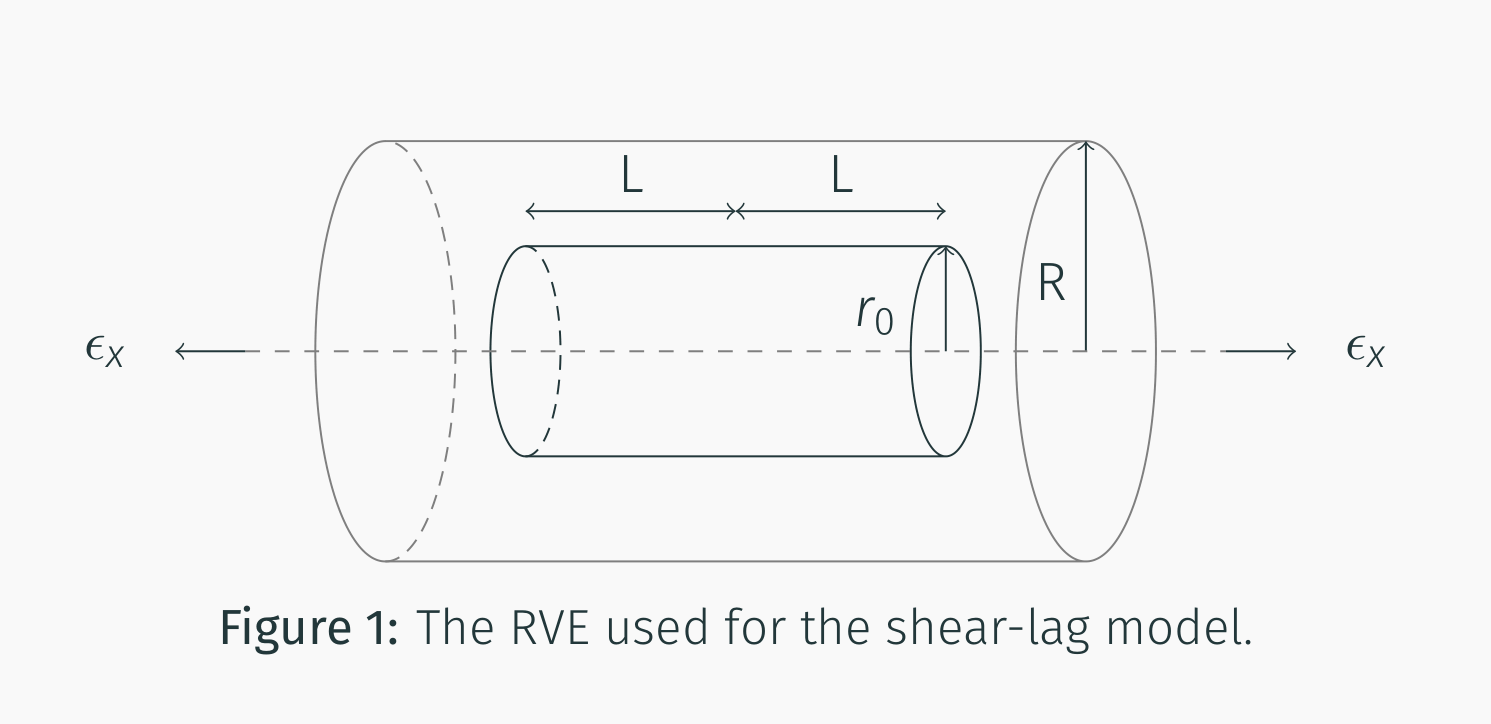
\includegraphics{../images/shearlag-intro.PNG}
\caption{shear lag diagram}
\end{figure}
\end{frame}

\begin{frame}{shear lag}
\protect\hypertarget{shear-lag-1}{}
\begin{itemize}
\tightlist
\item
  Balancing forces on a differential element we find
\end{itemize}

\[\begin{aligned}
  \sum F_x &= (\sigma_f + d\sigma_f) \frac{\pi d^2}{4} - \sigma_f\frac{\pi d^2}{4} - \tau_i (\pi d) dx = 0\\
  \frac{d\sigma_f}{dx} &= \frac{4\tau_i}{d}
\end{aligned}\]
\end{frame}

\begin{frame}{shear lag}
\protect\hypertarget{shear-lag-2}{}
\begin{itemize}
\tightlist
\item
  To integrate, we need to make some assumptions
\item
  It is commonly assumed that the normal stress on the end of the fibers
  is 0
\item
  Various assumptions are made about the shear stress, \(\tau\),
  Kelly-Tyson assumed it is constant (rigid plastic)
\item
  Cox assumed \(\tau\) is a linear function of \emph{x}
\end{itemize}
\end{frame}

\begin{frame}{shear stress}
\protect\hypertarget{shear-stress}{}
\begin{itemize}
\tightlist
\item
  We can also find the shear stress by comparing adjacent annuli of
  matrix material around the fiber
\item
  This assumes that fiber and matrix are perfectly bonded (continuous
  displacement at boundary)
\item
  The force balance due to shear in adjacent annula means that
\end{itemize}

\[ \pi d t = \pi d_0 \tau_i \]

\begin{itemize}
\tightlist
\item
  The shear stress far away from the fiber, \(\tau = G_m \gamma\), and
  if \(\\gamma = \frac{du}{dr}\), then we can say
\end{itemize}

\[\frac{r_0}{r} \tau_i = G_m \frac{du}{dr}\]
\end{frame}

\begin{frame}{shear stress}
\protect\hypertarget{shear-stress-1}{}
\begin{itemize}
\tightlist
\item
  We integrate to find that
\end{itemize}

\[\tau_i = \frac{G_m(u_R-u_f)}{r_0 ln(r)}\]

\begin{itemize}
\tightlist
\item
  Which we can substitute into our original force-balance equation to
  find
\end{itemize}

\[\frac{d\sigma_f}{dx} = \frac{4 G_m(u_R-u_f)}{ d r_0 ln(r)}\]

\begin{itemize}
\tightlist
\item
  But \emph{d}=2\emph{r}0, so we can simplify to
\end{itemize}

\[\frac{d\sigma_f}{dx} = \frac{2 G_m(u_R-u_f)}{ r_0^2 ln(r)}\]
\end{frame}

\begin{frame}{shear lag}
\protect\hypertarget{shear-lag-3}{}
\begin{itemize}
\tightlist
\item
  Finally, we differentiate with respect to \emph{x} to replace the
  displacements with strains
\item
  We assume that \emph{du}\emph{R}/\emph{dx} is far enough away from the
  fiber such that the strain is equal to far-field strain
\item
  The solution to the differential equation is
\end{itemize}

\[\sigma_f = E_f \epsilon_1 + B\sinh(nx/r) + D\cos(nx/r)\]
\end{frame}

\begin{frame}{stress in fibers}
\protect\hypertarget{stress-in-fibers}{}
\begin{figure}
\centering
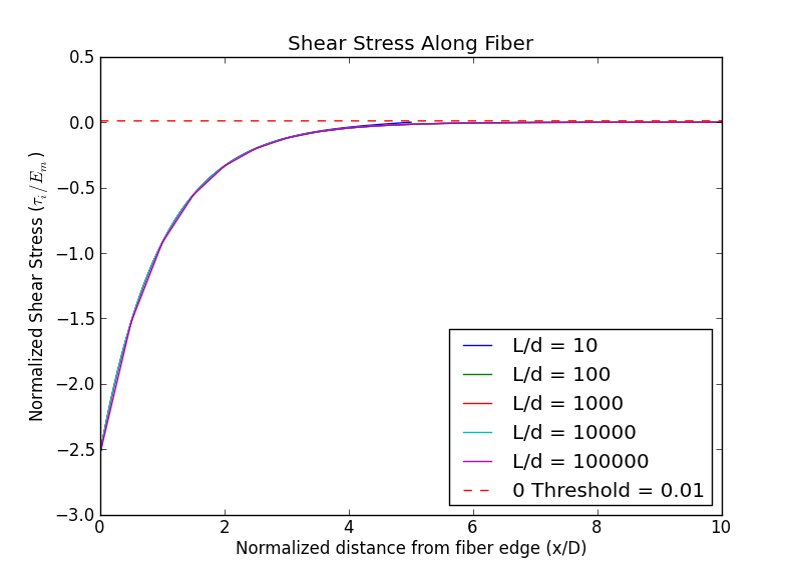
\includegraphics{../images/shearlag.png}
\caption{Stress near the edge of fibers in shear lag model}
\end{figure}
\end{frame}

\begin{frame}{normalizing}
\protect\hypertarget{normalizing}{}
\begin{itemize}
\tightlist
\item
  An interesting finding was that when we normalized distance (x) by
  fiber diameter
\item
  The shear stress was the same for any fiber length
\item
  This means that most/all shear stress transfer occurs near the ends
\item
  If fibers are not long enough, full stress profile does not develop,
  fibers contribute very little to stiffness
\end{itemize}
\end{frame}

\begin{frame}{next class}
\protect\hypertarget{next-class}{}
\begin{itemize}
\tightlist
\item
  Eshelby's equivalent inclusion
\item
  Textbook pages 94-99 and 364 - 370 (I feel these are pretty confusing
  though)
\end{itemize}
\end{frame}

\end{document}
